\chapter{Genetic architecture and landscape heterogeneity interact to determine adaptation during species range expansion}%The role of genetic architecture and environmental gradients in adaptation during range expansion}
\label{chap:heterogeneouslandscapes}

\section{Abstract}


\section{Introduction}

% speciation, local adaptation, range expansion are all about adaptation to novel environments
%	in particular, adaptation in the face of gene flow

% it is still today a major question in evolutionary biology what alleles contribute to local adaptation
% and equally unknown (?) and much more hotly debated is how many genes are needed for speciation to occur? few or many? or a whole genome? or one magic trait?

% by examining range expansion over different types of heterogeneous environments and with different underlying genetic architectures, we investigate the ability for populations to colonize new habitat and adapt in order to undergo a species range expansion


%discuss the question of adaptation broadly - it's important in many aspects of evolution
The question of why species range limits exist has pervaded evolutionary biology for decades. Understanding populations' abilities to adapt to novel environments is key to this process, and is a major area of study across evolutionary biology in studies of speciation, local adaptation, invasive species, and conservation biology. 
Populations are known to locally adapt within their species range to survive across a range of disparate environments \citep{Kawecki:2004}. On a more extreme scale, populations may eventually span such dissimilar environments that they reach a point of sufficient differentiation to produce new, isolated species adapted to different environments \citep{Rundle:2005, Doebeli:2003}. Adaptation to new environments determines the capacity of invasive species to thrive \citep{Prentis:2008}, and the potential for success of new genetic diversity from attempts of assisted migration \citep{Aitken:2013}. 
Regardless of whether adaptation results in the formation of new species or differentiated local populations, it remains a major question in evolutionary biology as to which and how many genes contribute to local adaptation. 

% talk about genetic architecture
Many studies, both empirical and theoretical, examine genetic architecture and its role in the ability to adapt to a novel environment \citep{Yeaman:2015, Yeaman:2011, Carroll:2001, Holloway:1990, Peichel:2001, Bratteler:2006, Schiffers:2014}. It is known that a sufficient level of genetic variation, $V_G$, is necessary to provide the alleles required for adapting to a new environment. It was previously thought that many alleles of too small an effect may be swamped by gene flow before being able to contribute to sufficient local adaptation, but as shown by \citep{Yeaman:2015}, this effect is possible through transient processes subject to random genetic drift when rates and sizes of mutations and genetic redundancy are sufficient (though detecting the presence of such alleles remains a difficult task). It is clear however, that fewer loci of larger effect can contribute best to adaptation, which eventually lead to the building up of linked clusters of locally adapted alleles, often referred to as genomic islands of divergence \citep{Feder:2010}. Even when small effect alleles may contribute to adaptation, larger effect alleles build up and contribute to adaptive differences among populations \citep{Yeaman:2011}. As \citet{Renaut:2013} have shown in sunflower, genetic architecture plays a larger role in contributing to genomic divergence than does the geography of speciation. %make sure to go back and see what they mean by this "geography"
The details of genetic architecture are thus vital in studies of adaptation, and should not, nor need not, be ignored in today's era of genomic technologies. % eh, maybe remove the last part here, I am only doing a simulation study after all

% talk about landscape heterogeneity - in broad terms
Whether a certain genetic architecture will successfully contribute to adaptation in a new environment will also depend largely on the environmental difference at hand. There are clearly biological limits that exist in terms of adapting to environments of extreme difference in optimal phenotype, but within the realm of biological reality, there may still be limits to the change in environmental optimum to which a given genetic architecture allows adaptation. In the real world, environments are heterogeneous, and they change in multifarious ways over space, from gradual to sudden, and of minor or major magnitudes of change. \citet{Schiffers:2014} have investigated the role of adaptation across patches of heterogeneous environment, but it has not yet been investigated how the degree of change in these optima will impact the outcome of adaptation during range expansion.
%The potential for genetic architecture underlying adaptation to interact with the environment to which populations are adapting is however less well understood. \emph{somewhere in here need to link better to the fact that I'm focusing on range expansions} %%

% talk about landscape heterogeneity in terms of range expansions
When considering environmental heterogeneity in terms of adaptation during range expansions, there are several important genetic processes that can lead to interesting hypotheses for adaptation across the landscape, making range expansions ideal for studying the combination of these effects. 
% Species exist on environmentally heterogeneous landscapes, and the degree of this heterogeneity can vary greatly within species ranges.
The characteristics of the environment available for a species to expand into plays an important role in the ability of populations to expand \citep{Aguilee:2012, Barton:2001, Pease:1989}. Increasing habitat heterogeneity, and thus heterogeneity in selective pressures, interacts with gene flow to influence the adaptive abilities of peripheral populations, and can in some cases inhibit local adaptation in peripheral populations \citep{Slatkin:1987,Kirkpatrick:1997, Ronce:2001}. During a range expansion, small founder populations at the margin experience reduced effective population sizes and reduced efficacy of selection. When this process repeats over the course of an expansion, the process of gene surfing \citep{Klopfstein:2006} can increase the presence of deleterious alleles and cause an expansion load at the range margin \citep{Peischl:2013}. This process is examined in more detail by Gilbert \emph{et al.} (\color{red} \footnotesize hopefully submitted \normalsize \color{black}). %or remove this sentence and just talk about dispersal?
Due to reduced density at range margins, these populations experience gene flow at much higher proportions than any populations existing within the denser core os the species range. This asymmetric migration can behave in two disparate ways: introducing new genetic variation needed for further adaptation in an otherwise genetically depauperate population, or swamping locally adaptive alleles with foreign maladaptive alleles thus preventing further adaptation. Which of these processes occurs will depend on the details of migration rates, mutation rates, population sizes, and the degree to which the environment differs across the species range.

Previous theoretical studies have examined many of these aspects and their role in local adaptation at range margins during the expansion process. Higher gene flow has been shown to introduce more maladaptive alleles from greater distances and thus be more detrimental to the local population \citep{GarciaRamos:1997}. While others have shown the effect of evolutionary rescue from migration when marginal populations have small effective population sizes and behave as sinks \citep{Holt:1997,Gomulkiewicz:1999,Ching:2012}. Alternatively, if selection is strong enough or migration reduced enough, this can prevent the establishment of foreign alleles in a population allowing it to adapt sufficiently to local conditions \citep{Ronce:2001}. 

Foundational work in the field showed that on a linear environmental gradient, increasing steepness of the change in environmental optimum eventually leads to maladaptation at the margin and eventual extinction of the species \citep{Kirkpatrick:1997}. %Improving upon this study by allowing realistic and evolving genetic variance showed no limits to adaptation at a range margin, and a wider range of results when investigating temporally changing environments and varying population densities \citep{ polechova
Further investigations have improved upon this and shown the effects of density dependent selection \citep{GarciaRamos:1997} as well as stochastic effects on low density \citep{Bridle:2010}, temporal changes in environments \citep{Pease:1989}, differing dispersal parameters \citep{Aguilee:2012}, evolution of genetic variance \citep{Barton:2001,Polechova:2009}, and the impacts of genetic drift  \citep{Polechova:2015} on adaptation or the lack thereof at range margins. %\citet{Case:2000} also incorporated species competition, under which they found similar results only with a shallower environmental gradient needed to limit range expansion. Some of these models use the same linear gradient of an environmental optimum changing at a constant rate over continuous space, while others simulate adaptation to differing environmental optima across discrete space (habitat patches) within which  individuals of a patch possess no explicit spatial designation. The results of these discrete environment models also show the potential for species to either adapt and persist, exist as non-adapted generalists, or go extinct.
%  **** include this and improve on the summary of other studies? --> One may predict that a given difference in optimum phenotype can be attained equally from few loci of large effect or many of small effect, but such a process will clearly rely on important details of migration, mutation, selection, and genetic drift. (cite someone here?) Strong asymmetric migration can swamp locally beneficial alleles and prevent adaptation (cite Kirkpatrick and barton, and others). Weak selection and strong genetic drift can prevent beneficial alleles from establishing (true??). And mutation may drive the presence of genetic variation needed to allow adaptation to novel conditions.
These studies have all largely investigated adaptation in models of two discrete habitat patches of different environmental optima or across linear gradients in continuous space. Yet both of these situations differ largely from biological reality, where environmental changes exist in some combination of these two layouts: contiguous space with varying levels of gradual or abrupt environmental changes distributed patchily across space. %may occur more or less frequently in space and to a greater or lesser degree of difference in phenotypic optimum. 
These differences in landscape play a key role in the process of populations adapting because of their potential to interact with the effects of evolutionary processes at the range margin. 

% set up our hypotheses/goals
When discrete habitat types exist contiguously across space, will the dynamics of the system reflect those of the continuous or the discrete models? %The combination of such environmental landscapes however, has not been sufficiently explored. 
\citet{Barton:2001} suggested the ability of populations to persist across environments of accelerating gradients, but in depth examination of different types of environmental heterogeneities is warranted. Because discrete models have as of yet not extended past two patches, it is unclear what effects a third or additional patches may have on evolution and adaptation within the system when space is explicit within each patch. With larger environmental differences in optima, will only large effect mutations be able to contribute to local adaptation and small effect alleles still swamped at the range margin?

% this project's hypotheses
In this study, we test if different genetic architectures and landscape heterogeneities can interact and affect the outcome of adaptation during a species range expansion, and potentially even limit a species range expansion. We compare our results to predictions from \citet{Barton:2001} and the results of \citet{Bridle:2010} and \citet{Schiffers:2014} to assess the impacts of our further explorations into genetic architecture and environmental heterogeneity. 
% how we're going to test those hypotheses
To address this question, we simulate a spatially explicit and discrete two-dimensional landscape across which populations expand their species range and adapt to newly encountered environments. We model a range of genetic architectures for a quantitative trait to test for differences in ability to adapt to environments. We also compare this across environments that differ in their degree of environmental heterogeneity from few to many locations of change in environmental optima, as well as in terms of the magnitude of change for each of these optima. Examining the rate of range expansion and the time required for populations to colonize and adapt in new environments provides insight into the role of both genetic architecture and environmental heterogeneity in determining the success or failure of adaptation. Such results are highly informative for the field of evolutionary biology, and largely applicable in predicting the fate of many species across the globe requiring the ability to adapt in the face of disturbance and shifting species ranges due to climate change and other anthropogenic environmental perturbations.


%<><><><><><><><><><><><><><><><><><><><><><><><><><><><><><><><><><><><><><>

% marginal populations thus often exist only as a sink, sustained by immigration until sufficient local adaptation is achieved. % and recovery from expansion load? -- refer to Ch 4 here, i.e. refer to our group project paper -- or just talk less about load since I'm not studying it in this paper
% When the population shifts to be a self-sustaining source, it escapes the effects of drift, and provides emigrants for further colonization and range expansion. This shift from sink to source also includes a shift away from asymmetric migration previously swamping locally adaptive alleles with foreign maladaptive alleles.

%Local adaptation within a species not only benefits populations in terms of fitness but also has repercussions for a species' global range. A species' range is defined in some cases by sharp visible boundaries, such as distinct geographical changes in landscape features, or equally understandable ecological reasons such as competitor occurrence or nutrient limitations. In instances where no such clear reason for a range edge exists, understanding what forces limit expansion and adaptation at the edge of a range becomes an evolutionary question \citep{Bridle:2007,Kawecki:2008,Excoffier:2009}. Barriers to dispersal may prevent expansion past the edge, however gene flow can also act to inhibit local adaptation in peripheral populations \citep{Slatkin:1987,Kirkpatrick:1997}. This, in combination with different selective forces from environmental gradients across the landscape, may prevent expansion. The characteristics of the environment available for a species to expand into plays an important role \citep{Aguilee:2012,Barton:2001,Pease:1989}. Increasing habitat heterogeneity, and thus heterogeneity in selective pressures, interacts with gene flow to influence the adaptive abilities of peripheral populations \citep{Ronce:2001}.

% Under one of the first models to examine the question of adaptation across species ranges \citep{Kirkpatrick:1997}, it was shown that three different scenarios could result: species extinction, a limited species range, or unlimited expansion of a species. Other studies have examined scenarios similar to this model and incorporated more realistic simulation methods that were previously not investigated: density dependent selection \citep{GarciaRamos:1997,Gomulkiewicz:1999} as well as stochastic effects on low density \citep{Bridle:2010}, temporal changes in environments \citep{Pease:1989}, differing dispersal parameters \citep{Aguilee:2012}, and evolution of genetic variance \citep{Barton:2001,Polechova:2009}. \citet{Case:2000} also incorporated species competition, under which they found similar results only with a shallower environmental gradient needed to limit range expansion. Some of these models use the same linear gradient of an environmental optimum changing at a constant rate over continuous space, while others simulate adaptation to differing environmental optima across discrete space (habitat patches) within which  individuals of a patch possess no explicit spatial designation. The results of these discrete environment models also show the potential for species to either adapt and persist, exist as non-adapted generalists, or go extinct.

%Equally relevant to studying adaptation in a local adaptation or speciation context, is the study of adaptation during a species range expansion. As a species range expands, it encounters novel habitat to which it must adapt. Previous studies have shown that it is the ability of populations at range edges to adapt to these new environments that can determine the ability of a range to expand (citations). Not unlike parapatric speciation, this adaptation to new environments must occur in the presence of gene flow. Asymmetric gene flow at a range edge, however, can cause migration load that is particularly strong when an edge population is still a sink and requiring the influx of individuals to persist.

%Species range limits and the capacity for range expansion has long been a question in evolutionary biology. A species' range is defined in some cases by sharp visible boundaries, such as distinct geographical changes in landscape features, or equally understandable ecological reasons such as competitor occurrence or nutrient limitations. In instances where no such clear reason for a range edge exists, understanding what forces limit expansion and adaptation at the edge of a range becomes an evolutionary question \citep{Bridle:2007, Kawecki:2008, Excoffier:2009}. Barriers to dispersal may prevent expansion past the edge, however gene flow can also act to inhibit local adaptation in peripheral populations \citep{Slatkin:1987, Kirkpatrick:1997}. This, in combination with different selective forces from environmental gradients across the landscape, may prevent expansion. 


%<><><><><><><><><><><><><><><><><><><><><><><><><><><><><><><><><><><><><><>



\section{Methods}

%\subsection{Simulation Model}

We model a species range expansion over heterogeneous environments with individual-based, forward time simulations in the program \textsc{nemo} \citep{Guillaume:2006} and vary two main parameters of interest: the genetic architecture underlying the quantitative trait, and the magnitude of change in environmental optimum in space. We also compare these effects across two cases of average dispersal distance. Our goal is to understand the impact and interactions of genetic architecture and the landscape heterogeneity over which individuals exist in terms of the outcome of range expansion and population adaptation.

We implement a modified version of \textsc{nemo} \citep{Guillaume:2006}, described in Gilbert \emph{et al.} (\color{red} \footnotesize hopefully submitted \normalsize \color{black}), which allows for a large-scale, two-dimensional species range to be modeled with explicit space. This expands greatly upon existing 2-patch models with non-explicit space within each landscape patch and approaches a model of continuous space. We initiate the population in a limited region for a burn-in to migration-mutation-selection equilibrium, after which populations expand into empty landscape of various environmental optima. Individuals are monoecious (hermaphroditic), obligately outcrossing diploids which possess a quantitative trait under balancing selection for the local environmental optimum. Generations are non-overlapping and life cycle events occurr in the order of breeding, dispersal, viability selection, and population regulation. We monitor the spread of individuals across the landscape in terms of speed and fitness as they encounter environments of differing environmental optima to which they must adapt in order to further expand.



% now go into all the gory details:
\subsection{Landscapes}

In order to approximate continuous space and maintain a spatially explicit landscape with discrete populations, we implemented a large spatial grid of habitat patches in \textsc{nemo}. This bridges the gap between existing two-patch landscape models, where existence within either of these two patches is not spatially defined, and models of continuous space, where \emph{\color{red} \footnotesize I still need to describe this  \normalsize \color{black}}. The landscape is a rectangular grid of $40\times2000$ cells with a defined phenotypic optimum for every cell in the landscape. Carrying capacity was regulated at $K = 5$ per cell. The burn-in period occurs in the leftmost $40\times40$ cells, after which expansion proceeds into the remaining $40\times1960$ cells. The burn-in area, hereafter termed the core, consistently possessed a constant optimum phenotypic value of 0 to ensure that the population was well-adapted before populations expanded onto the environmental gradients. In all cases, the environmental optimum only changed in one dimension over the axis of expansion (x-axis), and was constant over cross-sections of the landscape (y-axis). Terms for describing the simulation set-up and analysis are provided in Table \ref{tab:params}. Our landscape of $40\times2000$ cells also greatly builds upon the model of \citet{Schiffers:2014} which examined a grid of $16\times64$ cells.

We examined two % several
types of environmental heterogeneities across landscapes which can be defined by the number of changes in environmental optima that occur over space and the magnitude of these changes. We term each of these changes in optima on the landscape ``steps" because the environmental optimum is constant over space until it reaches a step where it then increases in magnitude to the new optimum which is then constant again until another step occurs. The magnitude of change in phenotypic optimum at a step is thus referred to as $h_{step}$ since it is the measure of the ``height" of a step. % should there be a supplemental fig that is a schematic of the landscape?
We compare the ability of populations to expand across environments that range from the extreme of one step in the landscape to the opposite extreme of a linear gradient. Because we are approximating continuous space with a grid, the closest our landscapes become to linear gradients are those where a step occurs between every cross-section.




%<><><><><><><><><><><><><><><><><><><><><><><><><><><><><><><><><><><><><><><><><><><><><><><><>
\begin{table}[h]
\centering \footnotesize
\caption{Terminology and parameter definitions for simulations}
\label{tab:params}
\begin{tabular}{lp{0.8\textwidth}l}
Term		& Explanation  \\ \hline \hline
Cell		& One unit of space on the landscape grid. 40 cells across the y-axis constitute a landscape cross-section. The entire landscape is $40\times2000$ cells.			\\ \hline
Core		& The leftmost $40\times40$ landscape cells. The population is limited to this region during the burn-in period. Environmental optimum is constant within the core.	\\ \hline
Step		& Used to describe an instance of a change in phenotypic optimum on the landscape.															\\ \hline
$h_{step}$ & The magnitude of change in phenotypic optimum across a step in the landscape. In other words, the height of a step.									\\ \hline
$h_{total}$ & The total magnitude of change in phenotypic optimum across the entire landscape. In other words, the sum of all step heights.							\\ \hline
Step width	& The number of landscape cross sections between subsequent changes in environmental optimum. In other words, the number of cross sections between each occurrence of a step in the landscape.	\\ \hline
\emph{K}	& Carrying capacity of a cell. Population regulation occurs at the level of cells. $K = 5$ in all cases.													\\ \hline
$\sigma_{breed}$ & One standard deviation of the Gaussian kernel describing the area of the breeding window. Individuals can find mates within cells contained by the breeding window. $\sigma_{breed} = 0.5\times$cell width in all cases. \\ \hline
$\sigma_{disperse}$ & One standard deviation of the Gaussian kernel describing the area of potential dispersal. Offspring can disperse to cells within the dispersal kernel. $\sigma_{disperse} = 2\times$cell width or $4\times$cell width as described in the text.                                          
\end{tabular}
\end{table}
%<><><><><><><><><><><><><><><><><><><><><><><><><><><><><><><><><><><><><><><><><><><><><><><><>




To first determine the factors underlying adaptation to a single, new environment, landscapes with one step were tested for $h_{step} = 5, 7.5, 10, 12.5,$ and $15$. In these cases, $h_{total}$ = $h_{step}$, and essentially mimics a spatially explicit 2-patch model. % For the same total change in optimum over the landscape, but at the other extreme of heterogeneity, i.e. being linear, populations had no difficulty in expanding to fill the landscape when $h_{total} \sim 0.0025, 0.005,$ and $0.0075$.
Upon determining the outcomes of success or failure to expand across this single step, we then simulated landscapes with increasing frequencies of steps, while holding $h_{step}$ constant at either 5 or 10, within each simulation. Step frequencies ranging from 4 to 1,959 (linear) steps per landscape were compared, which can equivalently be described as scenarios where the width of a step (the number of cross sections between subsequent steps) ranges from 392 cross sections down to a single cross section between steps on the linear gradient. Because $h_{step}$ is held constant in these scenarios, the total change in environmental optimum across the entire landscape, $h_{total}$, differs across cases of different step frequencies and is simply the product of $h_{step}$ and the number of steps on the landscape. The scenario for $h_{total}$ being held constant is not shown, since linear gradients with $h_{total} = 5, 10,$ or $15$ ($h_{step} = 0.0025, 0.005,$ or $0.0075$) posed no difficulty for any of our simulated populations to expand across and adapt (see Supplemental Figure \color{red}1\color{black}). 
% if I have time for the simulations, add in the description of non-monotonic step landscapes

% Multiple different scenarios can represent the same total change in landscape optimum (Figure 1a) while the frequency of steps in space can also result in different total changes in landscape optimum (Figure 1b).



\subsection{Breeding \& Dispersal \color{red} \footnotesize how much of the other paper should I reiterate? \normalsize \color{black}}
To maintain our spatially explicit approximation to continuous space, we introduced a breeding window into \textsc{nemo}. This allowed specification of a fine scale landscape to underly larger populations. The breeding window defines a given radius of cells around a focal cell from which an individual can find a potential mate during the breeding life cycle stage and is described in detail in Gilbert \emph{et al.} (hopefully submitted). 
% Upon mating, offspring are then placed in the mother's cell, after which dispersal would proceed as normal in the subsequent life cycle event. Within this radius, individuals present are chosen as a mate with decreasing probability away from the focal cell. This radius and the mating probabilities are determined by a continuous, Gaussian distribution that is discretized by the probability density within each cell. 
The probability of finding a mate is described by an approximate bivariate Gaussian defined by one standard deviation of a Gaussian distribution, $\sigma_{breed}$, where $f(x,y) \propto \exp{[-(\frac{\Delta x^2}{2\sigma_{breed}^2}+\frac{\Delta y^2}{2\sigma_{breed}^2})]}$ gives the distance traveled to search for a mate in a given direction $x$ and $y$. The maximum search radius for a mate is limited to $4\times\sigma_{breed}$. $\sigma_{breed}$ was set at one half of a cell size. This produced a breeding window containing the 12 cells surrounding the focal cell. Because modeling a range expansion implies that there will often be lone colonists on the expansion front, this addition of a breeding window increases biological realism by allowing lone colonists on the range front to still potentially find a nearby mate, even if they are the sole inhabitant of their cell. This most closely resembles obligately outcrossing plants, who may receive pollen from nearby mates, but could also represent animals that search for mates nearby then return to their home territory. Individual fecundity was drawn from a Poisson distribution with mean 4 to determine the number of offspring to be produced.

Dispersal occurred similarly to breeding, where a dispersal kernel was defined for forward rates of migration and discretized over cells on the landscape. This distribution was defined by $\sigma_{disperse} = 2\times$ cell size for the majority of simulations. Where specified, a larger dispersal kernel of $\sigma_{disperse} = 4\times$ cell size was implemented. An R wrapper package was created to calculate breeding and dispersal kernels, and to discretize these probabilities across the landscape, and is available online at https://github.com/kjgilbert/aNEMOne. C++ code for the modified version of \textsc{nemo} with a breeding window is available online at https://github.com/kjgilbert/NemoDispersalKernel.
 
 
 
\subsection{Genetic Architecture}
The quantitative trait, $z$, is underlain by 100 freely recombining loci. We held the total mutational variance, $V_m$, available to the system constant at $10^{-2}$, but varied the underlying genetic architectures contributing to the mutational variance. The number of loci, $L$, was also held constant at 100, thus to satisfy $V_m = 2 L \mu \alpha^2$, we varied the per locus mutation rate, $\mu$ and the variance in mutational effect sizes, $\alpha^2$. 
Four genetic architecture regimes were investigated as follows. First, one with small effect mutations and a higher mutation rate: $\mu = 10^{-2}$ and $\alpha^2 = 0.005$. Second and third intermediate regimes set $\mu = 10^{-3}$ and $\alpha^2 = 0.05$, and $\mu = 10^{-4}$ and $\alpha^2 = 0.5$. The fourth regime allowed for the largest effect mutations to occur proportionally more often, yet exhibit less frequent mutations overall where $\mu = 10^{-5}$ and $\alpha^2 = 5.0$. 



\subsection{Viability Selection}
Selection occurs only on survivorship throughout the simulations. Selection is stabilizing for the phenotypic optimum, with fitness of an individual is defined by $\omega_z = exp[-\frac{(z-z_{opt})^2}{2V_S V_E}]$ \color{red} \footnotesize check it's right I put Ve on the bottom here \normalsize \color{black}  , where $z$ is the quantitative trait value, $z_{opt}$ is the optimum phenotypic trait for a given cell on the landscape, and $V_S$ is the selection variance. We set $V_S = 7.5$, and environmental variance, $V_E$, was set to 1. This matches the choice of $V_S$ and $V_E$ in Gilbert \emph{et al.} (\color{red} \footnotesize submitted AKA, chap 4 \normalsize \color{black}) which was derived from Kingsolver \emph{et al.} (2001) and Johnson and Barton (2005).
 
 
 

% A 1-dimensional probability distribution is drawn, defined by one standard deviation of a Gaussian distribution $\sigma$, which is then multiplied by itself to create a 2-dimensional kernel. This is reduced to include only probabilities equal to or higher than the smallest probability from the 1-dimensional kernel, and is then renormalized. 


%Figure 1 - Visualizations in 1-dimension of heterogeneously changing environmental gradients. Each horizontal portion is referred to in the text as a step. $h_{step}$ is a measure of the vertical distance between steps while $h_{total}$ is the total change in environmental optimum from one end of the landscape to the other. Panel A shows gradients that have the same overall slope, b ($h_{total}$ = 200), but different magnitudes of change in the local optimum, $h_{step}$. Panel B shows gradients that have different overall slopes, b, but the same magnitude of change in the local optimum per step ($h_{step}$ = 4).




\section{Results}

\subsection{Single step environmental changes}
% where did range limits form? (what parameter cases?) figure on wait times
A single step in the environmental optimum, analogous to two patches of different habitat on the landscape, prevented expansion and adaptation into the second habitat in cases where the magnitude of $h_{step}$ ($= h_{total}$) was too large. The cases where this magnitude was too large, however, varied across our cases of genetic architecture. This is measured in terms of the time during which populations have reached the location of the change in environment on the landscape (step), but remain stationary before expanding across the remainder of the landscape (Figure \ref{fig:wait1step}).

\begin{figure}[h]
\centering
\makebox[\textwidth]{
        \includegraphics[width=1\linewidth]{wait_times.pdf}}
\caption[Wait times for step crossing.]{Wait times in generations for step crossing over 1 step in the environment for each regime of genetic architecture simulated and across varying magnitudes of step height. Points are jittered for visualization.}
\label{fig:wait1step}
\end{figure}


This shows the trend that increasing the height of a step makes adaptation to the new environment increasingly more difficult, but also interestingly shows that different genetic architectures can contribute to successful expansion and adaptation in different ways. We find that decreasing the mutation rate increases the time taken to adapt to the new environment up to the point where adaptation is no longer attainable. However, in the case of the lowest mutation rate, having a large variance in mutation effect size counteracts this effect.
% show standing genetic variance during burn-in that allows expansion from Vg but not from low mutation rates
We can clearly see that the equilibrium level of genetic variance present in populations varies dependent solely on the mutation rate $\mu$, not on the variance in mutational effect size (Figure \ref{fig:va}). However, unlike previous predictions, the genetic variance present in the system is not necessarily determinant on the outcome of expansion and adaptation. Few, but large effect mutations can occur that equivalently provide the ability to survive in a newly encountered habitat. Adaptation under this regime requires more time to expand, since the requisite mutations for survival in the new environment must occur at or near the location of the environmental step.

\begin{figure}[h]
\centering
\makebox[\textwidth]{
        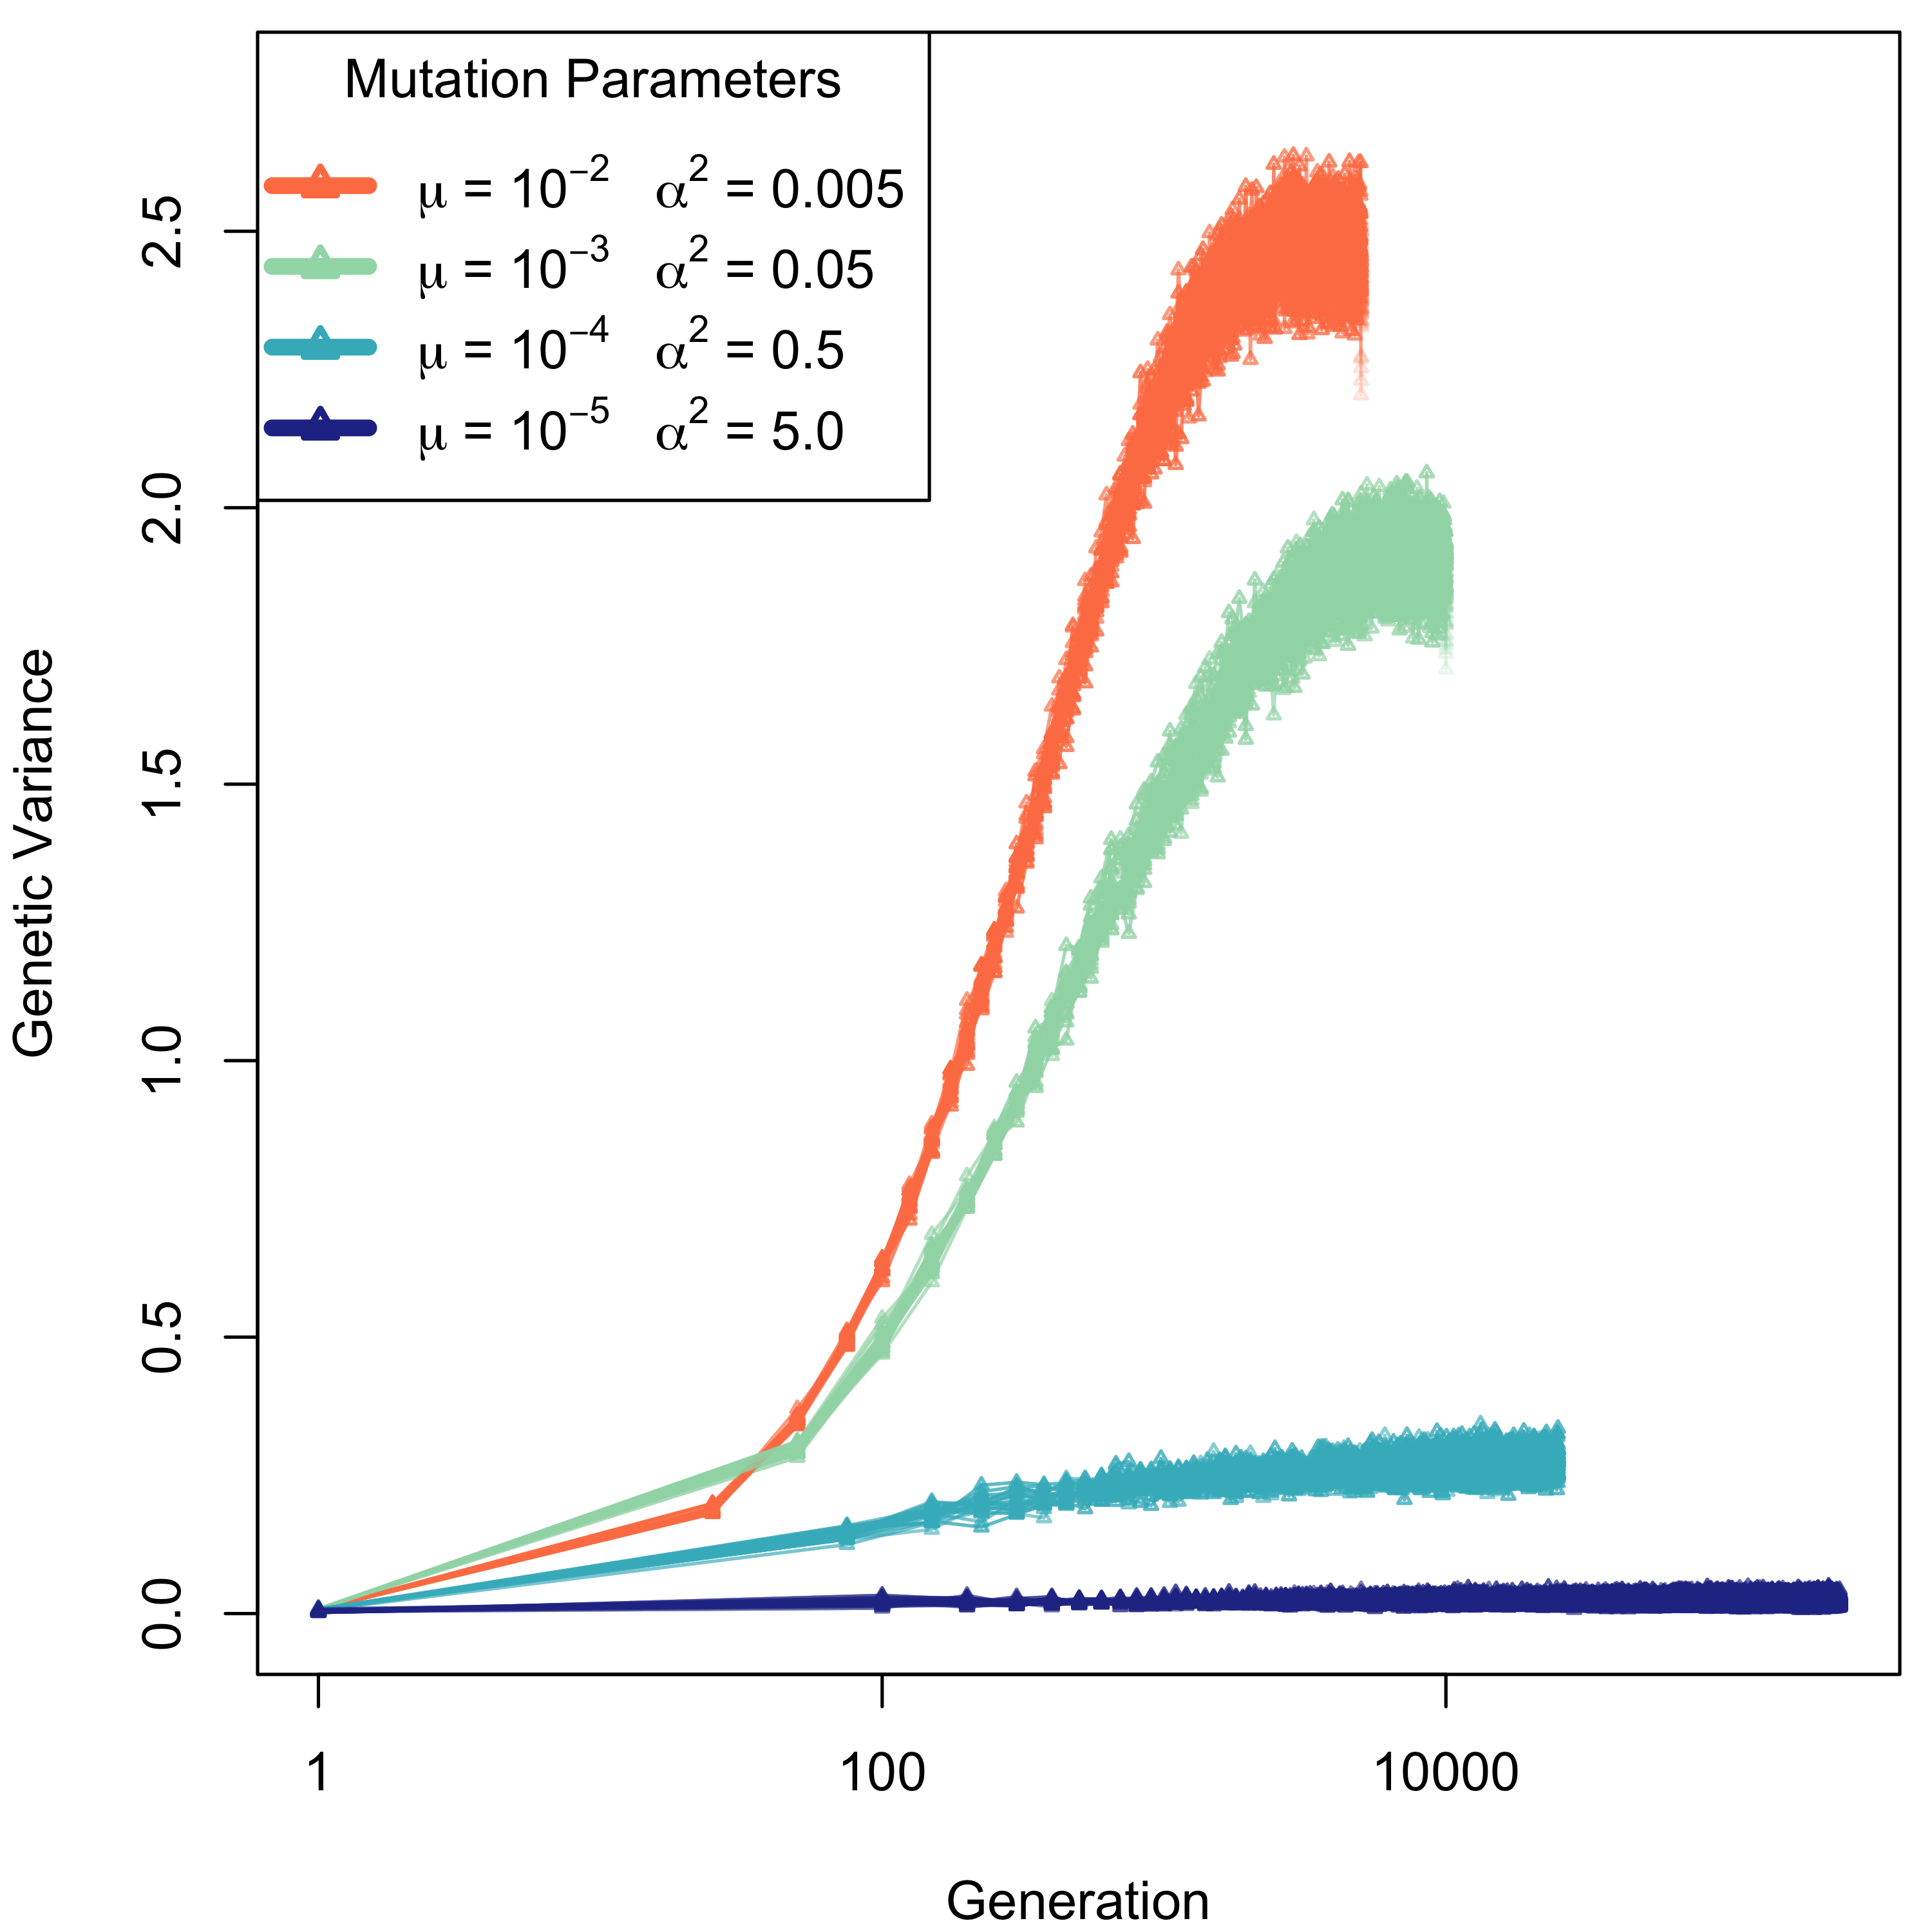
\includegraphics[width=0.6\linewidth]{CompareVa_OnePlot.png}}
\caption[Genetic variance during burn-in.]{Genetic variance during the burn-in period for each genetic architecture regime. All 20 replicates are plotted for each case.}
\label{fig:va}
\end{figure}

% genetic variance is inflated at each step to allow for adaptation across (need to add this as a figure?)
\color{red} \footnotesize \emph{Not sure if it's worth mentioning here or just in supplement:} Across the landscape, genetic variance remains at equilibrium after the expansion has completed, except at the step in environmental optimum, where variance is inflated due to migration from either disparate environmental optimum across this step (make a figure for this?). \normalsize \color{black}

% show effect size comparisons across loci that show larger effect mutations occurring in larger variance cases
We confirm the causal factor of large effect mutations contributing to adaptation across the setup under our fourth genetic architecture regime by comparing the %mutations that have contributed to adaptation across the step in environmental optimum, we examine the 
per-locus differences in mean genotypic value below and above the environmental step. We do this within \color{red}XX \color{black} generations of the expanding front passing this point on the landscape in order to capture the mutations directly contributing to adapting to the novel environment, rather than mutations that build up over time during further adaptation to each respective environment. This comparison is made between the 20 cross sections closest to and below the step and the 20 closest cross sections above the step, excluding the 2 cross-sections immediately adjacent above and below the step, as these are mostly inflated by local gene flow. We find that in the cases where a larger variance in mutational effect was specified, adaptation to the new environment is due to fewer loci of larger effect, even though an identical number of loci are available in the system (Figure \ref{fig:effect_sizes}). Larger differences in per-locus effects are particularly true when adaptation to the new environment is more difficult ($h_{step}$ is larger), showing the increased contribution of few large-effect loci to successful expansion into the new environment.


\begin{figure}[H]
\centering
\makebox[\textwidth]{
        \includegraphics[width=1.1\linewidth]{effect_sizes.pdf}}
\caption[Per locus effect size differences.]{Per locus effect size differences below and above the environmental step. All 20 replicates are plotted for each case, meaning that counts sum to 2000 per scenario. \color{red} \footnotesize this is rough; I'll fix the x-axis and layouts and label the counts going off the screen  \normalsize \color{black}}
\label{fig:effect_sizes}
\end{figure}


% effects of larger dispersal kernel
We briefly compare these processes under a condition of 2-fold increased dispersal. These results show increasing difficulty to adapt to the new environment (in all but one case which may not be significantly different: $\mu = 10^{-3}, \alpha^2 = 0.05$), with the similar trend where cases of higher mutation rate are more easily able to cross the environmental step. Wait times are increased on average, and previous cases that succeeded in adapting and expanding are no longer able to do so (see Supplemental Figure \ref{fig:wait1step2}). This evaluation needs further investigation of additional dispersal parameters for thorough understanding, as described in the Discussion.

\begin{figure}[h]
\centering
\makebox[\textwidth]{
        \includegraphics[width=1\linewidth]{wait_times2.pdf}}
\caption[Wait times for step crossing with increased dispersal.]{Wait times in generations with dispersal increased 2-fold for step crossing over 1 step in the environment for each regime of genetic architecture simulated and across varying magnitudes of step height. Points are jittered for visualization.}
\label{fig:wait1step2}
\end{figure}

\emph{NB it is possible that more dispersal is resulting in more swamping of the beneficial large effect mutations, and seems like a possible cause from the results on per-locus effect size differences, but not sure I've got enough evidence to say this.} %Fewer large effect mutations are seen having arisen, presumably due to more swamping preventing them from establishing, and preventing successful adaptation. % but remember, I have no expansion in some of these cases, so hard to say if they ever arose in the first pace? no- they must have because all else is the same


% how did this compare to previous predictions?
We can compare our results of successful adaptation or prevented expansion to predictions from \citet{Barton:2001} and \citet{Bridle:2010}. \citet{Barton:2001} predicts the critical gradient value from a 2-allele model to exist where within one dispersal distance, $b_{crit} = \sqrt{\frac{4 V_G}{\sigma^2 \gamma}}$, where $b$ is the slope of the gradient, and $V_G$ is the total genetic variance, $\sigma^2$ the variance in dispersal distance, and $\gamma$ a measure of the weakness of density-dependent regulation. %$V_G = b \sigma \sqrt{V_S}$, where $b$ is the slope of the gradient, and $V_G$ is the total genetic variance. 
Equivalently, \citet{Bridle:2010} reformulate this, given the assumption that $V_G = b \sigma \sqrt{V_S}$, as a critical gradient of $b > \frac{2 r_m \sqrt{V_S}}{\sigma}$ resulting in extinction, where $r_m$ is the maximum population growth rate. We do not simulate logistic growth, as is done in these previous works, but the maximum population growth rate is approximately similar to the logistic, where at low density, fecundity is equal to the maximum growth rate, and at high density this maximum rate decreases as there is limited space on the landscape for individuals to exist. Following from \citet{Bridle:2010} (I'll have to put more thought into the Barton comparison), we would expect our critical gradient value, $b$, to exist at approximately $h_{total} = 10.79$ for our smaller dispersal kernel and at $h_{total} = 5.46$ for our larger dispersal kernel. % 2 * 4 * sqrt(7.5)  / (2+0.5) = 8.76356  OR for disp 200: 2 * 4 * sqrt(7.5)  / (4+0.5) = 4.868645 BUT if TD = sqrt(sigms_disp^2 + 0.5* sigma_breed^2) then... first bcrit = 10.7872 and second bcrit = 5.4559
These predictions are broadly met for out smaller dispersal kernel, where expansion occurs below $h_{step}$ ($= h_{total}$) of 10, as well as at 10 for all but our third genetic architecture regime. Results of our larger dispersal kernel, however, do not meet these predictions where expansion occurs at much larger step heights.

On a linear gradient for the same $h_{total}$ as these single step environments, range expansion is not limited, and adaptation occurs across the landscape (Supplemental figures xxx). % (\color{red}maybe put these figures back in now that I think of it?\color{black}). 
But in the extreme case where environmental change is concentrated to one location in the landscape, we have shown that adaptation becomes too difficult. In this case, it is clear that overall gradient of the landscape is not a useful indicator of the outcome for range expansion. However, as we investigate next, it is also clear that the magnitude of change in environmental optimum, $h_{step}$ is alone also not a sufficient determinant of the outcome of range expansion.%maybe move this to the end just before I start describing the multistep cases?

% all else equal just increasing mutation rate always makes it easier to cross a step



\subsection{Multiple step environmental changes}

The ability to adapt to one new environment, i.e. cross one environmental step, does not necessarily imply the ability to adapt to many. We next investigated range expansion across environments of multiple sequential steps, each time increasing the environmental optimum by $h_{step}$. This is examined only for two cases: $h_{step} = 5$ where the one-step case resulted in adaptation and expansion in every case without hesitation, and $h_{step} = 10$ where the one-step case resulted in a limited subset of scenarios for successful adaptation and expansion. In these multi-step cases, steps were placed evenly across the landscape at frequencies ranging from only 4 steps on the entire landscape, up to 1959 steps (a linear gradient beyond the landscape core). $h_{total}$ is thus a product of $h_{step}$ and the number of steps occurring.

% just because you can cross one step, doesn't mean you can cross many
We found no cases where expansion succeeded over some, but not all steps on the landscape. In other words, when expansion did not occur, only sink populations were able to exist beyond the landscape core and the formation of a new range edge beyond this did not occur. %%%%%%\color{red} \footnotesize make sure this is true, don't think I've actually checked  \normalsize \color{black}.

% in what multistep parameter cases were there stable range limits?

When the total landscape gradient is made up of shallower steps ($h_{step} = 5$), the limit at which expansion no longer occurred was at a much higher $h_{total}$ than when the landscape is made up of steeper steps (Figure \ref{fig:multistep}). This again supports the point that total gradient value cannot alone accurately predict range expansion. We can further see from Figure \ref{fig:multistep} that the larger dispersal kernel leads to faster expansion with fewer steps when $h_{step} = 5$, but crosses a threshold where its expansion speed quickly slows and drops to zero, while the smaller dispersal kernel is still able to expand and adapt on a slightly steeper gradient. This effect can be attributed to the increased migration load that results from immigrants native to different steps introducing locally maladaptive alleles, and when dispersal allows for individuals to migrate further, this happens sooner as the frequency of steps increases (step width decreases). We see this reflected in the higher genetic variance present at the steps, and the inflation of this variance between steps when step width is reduced (need to make this figure still). This leads to local maladaptation and local extinction.

\begin{figure}[H]
\centering
\makebox[\textwidth]{
        \includegraphics[width=0.9\linewidth]{Rough_MultistepExpansionSpeeds.pdf}}
\caption[Rate of expansion for multi-step landscapes.]{Rate of expansion for multi-step landscapes across regimes of genetic architecture. \color{red} \footnotesize I will make this figure much better in the future - more data is incoming (probably want to do the mean w/ error bars and connect with lines) \normalsize \color{black}}
\label{fig:multistep}
\end{figure}

I would put a paragraph here on comparing the limit of no expansion in multi-step cases to predictions from Barton.

% can we see why

% what is the step width relative to the step height where the limit is?
% what is the total gradient relative to mutation parameters where the limit is?
% i.e. is is step width or is it just total gradient?

% figure for expansion rate across cases and step heights

% fitness and genetic variance results


\subsection{Non-monotonic changes in environment}
I am considering running a set of simulations where steps do not increase monotonically, but might increase then decrease again then increase again. Perhaps some genetic architectures might better pre-adapt populations to future steps to be encountered.
% is expansion speed faster when non-monotonic?
% is fitness higher?
% could this be due to pre-adaptation to future environments?


	

%%The slowed expansion is due to several factors. When steps are too frequent in space, there is insufficient space for individuals to adapt to their local optimum without migrants from nearby steps contributing maladaptive individuals. This is shown by mean fitness values averaged across the center of steps decreasing as step frequency increases, and by genetic variance averaged across the center of steps increasing as step frequency increases (Figure 5).



%%Causes (?) of success/failure to expand
%%As shown in figure 5, as steps increase in frequency across the landscape, genetic variance increases and fitness decreases. These qualities are the defining factors in determining whether populations are able to adapt and expand over changes in the environment (cite all the papers where too high genetic variance = extinction, but probably move this to discussion). Too high genetic variance results in maladaptation to the local optimum, decreased fitness, and eventually in local extinction. However, returning to the cases where there is only one step where the environmental optimum changes, we find that there is also a minimum amount of genetic variance necessary to adapt to new environments (Figure 6). When the hstep is smaller, less drastic mutations are required to survive across the step, so genetic variance does not become greatly increased (red lines Fig 6). As hstep increases, increasingly different genotypes are necessary to survive in the new environment, inflating genetic variance at the location of the environmental change as populations adapt to either side. When hstep is too large, the necessary mutations are not seen arising in the population, and individuals beyond the step are only a sink population and still adapted to the environment before the step, maintaining a low genetic variance.


%To do: the cases in blue in fig 6 need to be scrutinized further. What mutations arise right when they start to expand? The mutations that arise in populations at the step� look at their effect sizes, look at how many it takes

\section{Discussion}

Because previous studies (citations) found the steepness of the environmental gradient to determine ability to expand, %as was recapitulated here, 
we further investigated the underlying factors that impact this ability. This was done by teasing apart the effects of absolute magnitude of change in environmental optimum and the frequency of this change over space. As we have shown, on a linear gradient where expansion for a given parameter set is able to expand, e.g. $h_{total} = 15$, the same parameter set can no longer expand when the environmental change is reorganized into one step in the landscape. % I HAVE TO SHOW THE LINEAR CASE IF I SAY THIS HERE

The ability to cross a single step in the landscape is driven by the mutations available to the system. Sufficient small effect mutations contributing to standing variation can allow for adaptation to a new environment, while few mutations of larger effect can also allow populations to adapt to the new landscape optimum and spread across the remainder of the landscape. This latter regime can involve much longer times before adaptation occurs and expansion proceeds. 
\color{red} Discuss relation to Gomulkiewicz source-sink literature \color{black} %This result is similar to that of Gomulkiewicz (citation) where instead a 2-patch model is simulated, and the second patch switches from a sink to a source when 

Interestingly however, the ability of a parameter set to cross a single step does not guarantee its ability to cross multiple steps. In these cases, the frequency of steps occurring over the landscape drives the ability of populations to expand and adapt. This is due to...


\section{Acknowledgements}
We would like to thank Fred\'eric Guillaume for help with \textsc{nemo} and members of the Whitlock lab for comments and feedback.


%%% Local Variables:
%%% TeX-master: "thesis"
%%% TeX-PDF-mode: t
%%% End:
